\section{Differential Geometry}
\subsection{Vectors}
In order to look at vectors in a more general space we need to consider our vectors as something seperate from a line segment in flat space.
If we consider a function $f(x^\alpha)$ and a curve $x^\alpha(\sigma)$. The derivitive is therefore defined as:
\begin{align*}
	\frac{df}{d\sigma} &= \lim_{\epsilon\to0} \frac{f(x^\alpha(\sigma + \epsilon) - f(x^\alpha(\sigma)}{\epsilon} \\
	\frac{df}{d\sigma} &= \frac{dx^\alpha}{d\sigma} \partder{f}{x^\alpha}
\end{align*}
We then define our vector tangent to this curve $t^\alpha = \frac{dx^\alpha}{d\sigma}$. This mapping between directional derivatives and vectors is a 1-1 correspondance.
For any vector $a^\alpha$ corresponding to a directional derivitive we can write this as:
\begin{align*}
	\bm{a} &= a^\alpha \partder{}{x^\alpha}
\end{align*}
Where these partial derivitives now take the role of basis vectors. This correspondence between our basis vectors and our directional derivatives gives us a way of calculating basis transformations:
\begin{align*}
	\bm{a} &= a^\alpha \partder{x'\ ^\beta}{x^\alpha} \partder{}{x'\ ^\beta} \\
	a'\ ^\beta &= \partder{x'\ ^\beta}{x^\alpha} a^\alpha & a^\beta &= \partder{x^\beta}{x'\ ^\alpha} a'\ ^\alpha
\end{align*}

\subsection{Dual Vectors}
A dual vector is a linear map from vectors to real numbers. The real number that $\bm{\omega}$ maps $\bm{a}$ to is called $\omega(\bm{a})$. This should obey:
\begin{align*}
	\omega(\alpha \bm{a} + \beta\bm{b}) &= \alpha\omega(\bm{a}) \beta\omega(\bm{b})
\end{align*}
This can be represented as $\omega(\bm{a}) = \omega_\alpha a^\alpha$ clearly in order to obey all our linearity constraints. $\omega_\alpha$ are called the components of our dual vector.
We can say that the gradient of a function is a dual vector. If we recall that the derivitive of a function specifies a tangent vector $\bm{t}$, Then our gradient becomes:
\begin{align*}
	\partder{f}{x^\alpha}t^\alpha
\end{align*}
Where the $t^\alpha$ is a vector and $\partder{f}{x^\alpha}$ is our dual vector.

We can tell that clearly a set of four linearly independant dual vecotrs $\bm{e}^\alpha$ will provide a basis for all dual vectors:
\begin{align*}
	\bm{\omega} &= \omega_\alpha \bm{e}^\alpha
\end{align*}
Where these have been related to our normal basis vectors via:
\begin{align*}
	e^\alpha(\bm{e}_\beta) &= \delta^\alpha_\beta
\end{align*}

Putting this together we see:
\begin{align*}
	\omega(\bm{a}) &= \omega_\alpha e^\alpha(a^\beta\bm{e}_\beta) \\
	\omega(\bm{a}) &= \omega_\alpha a^\beta e^\alpha(\bm{e}_\beta) \\
	\omega(\bm{a}) &= \omega_\alpha a^\beta \delta_\beta^\alpha \\
	\omega(\bm{a}) &= \omega_\alpha a^\alpha
\end{align*}
\subsection{Correspondence between vectors and dual vectors}
Given a coordinate basis we can say:
\begin{align*}
	\bm{e}_\alpha(x)\cdot\bm{e}_\beta(x) &= g_{\alpha\beta}(x) \\
	\bm{a}\cdot\bm{b} &= g_{\alpha\beta} a^\alpha b^\beta
\end{align*}
So:
\begin{align*}
	a_\alpha &= g_{\alpha\beta}a^\beta
\end{align*}
We can then define an inverse metric such that:
\begin{align*}
	g_{\alpha\beta}g^{\beta\gamma} &= \delta_\alpha^\gamma \\
	a^\alpha &= g^{\alpha\beta}a_\beta
\end{align*}
If we have an orthonormal basis where $g_{\alpha\beta} = \eta_{\hat{\alpha}\hat{\beta}}$ then:
\begin{align*}
	a_{\hat{0}} &= - a^{\hat{0}} & a_{\hat{i}} &= a^{\hat{i}}
\end{align*}
We can use our basis vectors to project to components:
\begin{align*}
	\bm{e}^\alpha \cdot \bm{a} &= \bm{e}^\alpha\cdot a^\beta \bm{e}_\beta \\
	\bm{e}^\alpha \cdot \bm{a} &= a^\beta \bm{e}^\alpha\cdot \bm{e}_\beta \\
	\bm{e}^\alpha \cdot \bm{a} &= a^\beta \delta^\alpha_\beta \\
	\bm{e}^\alpha \cdot \bm{a} &= a^\alpha
\end{align*}
If we know the components $a^\alpha$ of a vector in a corrdinate bassis, then if we can say our coordinate basis components of orthonormal basis vectors and our dual basis are known then we can find our orthonormal components:
\begin{align*}
	a^{\hat{\alpha}} &= (e^{\hat{\alpha}})_\alpha a^\alpha & a_{\hat{\alpha}} &= (e_{\hat{\alpha}})^\alpha a_\alpha
\end{align*}

Taking as an example skew rectangular coordinates in flat space. In these coordinate $x$ and $y$ are not orthogonal and instead have an angle $\psi$ between them. We have a line element:
\begin{align*}
	dS^2 &= dx^2 + 2\cos\psi dxdy + dy^2
\end{align*}
We can see that clearly our dual basis vectors must be orthoogonal to the basis vectors they aren't associated with.
We can see that the lengths of the dual vectors can (and in general must) be non-unit in order to have our orthogonal relationships.
\begin{figure*}[h]
	\centering
	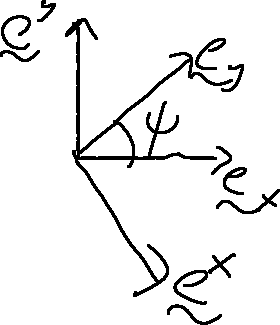
\includegraphics[width=12cm]{2-27-1.png}
	\caption*{Skew rectangular coordinates}
\end{figure*}

We now look at the example of normal vectors in 3-D space. Given a 3-surface in 4-D spacetime. 
We define the 3-surface in  terms of a function that is constrained, i.e. $f(x^\alpha) =\text{const}$. The gradient of $f$ will provide a normal vector:
\begin{align*}
	n_\alpha &= \partder{f}{x^\alpha}
\end{align*}
\subsection{Tensors}
We say that a vector is a bilinear (or more) map from pairs (or more) vectors into real numbers.

The metric is the tensor that maps two vectors into their inner product:
\begin{align*}
	g(\bm{a},\bm{b}) &= \bm{a}\cdot\bm{b}
\end{align*}
A rank r tensor is a r-linear map from r vectors to $\mathbb{R}$. We can write the tensor in terms of either the vector or dual vector basis. We can see:
\begin{align*}
	t(\bm{a},\bm{b},\bm{c}) &= t_{\alpha\beta\gamma} a^\alpha b^\beta c^\gamma \\
	t(\bm{a},\bm{b},\bm{c}) &= t_{\alpha\beta\gamma} a^\alpha b^\beta g^{\gamma\delta}c_\delta \\
	t(\bm{a},\bm{b},\bm{c}) &= t_{\alpha\beta}^{\ \ \gamma} a^\alpha b^\beta c_\gamma \\
	t_{\alpha\beta\gamma} &= t_{\alpha\beta}^{\ \ \delta}g_{\gamma\delta}
\end{align*}
And so on and so forth, we can change our representation to have any mix of upper and lower components using the metric.
We can also see that this gives us a mechanism to use tensors to map other tensors into other tensors, ex:
\begin{align*}
	v_\alpha &= t_{\alpha\beta\gamma} a^\beta b^\gamma
\end{align*}
If we sum upper and lower indicies, we call it a contraction (or sometimes a trace), ex:
\begin{align*}
	\omega_\alpha &= t_{\alpha\beta}^\beta
\end{align*}
Notably some objects that initially look like tensors (like Christoffel symbols) do not behave like tensors.
\subsection{Converting Tensor Components}
We want to look at converting our tensor components from coordinate basis to orthonormal basis.
We can describe any rank two tensor in terms of two vectors:
\begin{align*}
	t_{\alpha\beta} &= u_\alpha v_\beta
\end{align*}
We know that our orthonormal components can be calculated by:
\begin{align*}
	u_{\hat{\alpha}} &= (e_{\hat{\alpha}})^\alpha u_\alpha
\end{align*}
So:
\begin{align*}
	t_{\hat{\alpha}\hat{\beta}} &= (e_{\hat{\alpha}})^\alpha (e_{\hat{\beta}})^\beta u_\alpha v_\beta \\
	t_{\hat{\alpha}\hat{\beta}} &= (e_{\hat{\alpha}})^\alpha (e_{\hat{\beta}})^\beta t_{\alpha\beta}
\end{align*}

If we now look at going between different coordinate basis $x^\alpha$ and $x'\ ^\alpha$. Clearly we know:
\begin{align*}
	a_\alpha b^\alpha &= a'_\beta b'\ ^\beta \\
	a^\beta &= \partder{x^\beta}{x'\ ^\alpha}a'\ ^\alpha & a'_\beta &= \partder{x^\alpha}{x'\ ^\beta}a_\alpha
\end{align*}
And so we can write:
\begin{align*}
	g'_{\alpha\beta} &= \partder{x^\gamma}{x'\ ^\alpha} \partder{x^\delta}{x'\ ^\beta} g_{\gamma\delta} \\
	t'_\beta\ ^\alpha &= \partder{x'\ ^\alpha}{x^\gamma}\partder{x^\delta}{x'\ ^\beta} t^\gamma_\delta
\end{align*}
\subsection{Derivatives of vectors in curved space}
We have established that the partial derivitive of a function $f$ will give us a (dual) vector $\del f$ with components:
\begin{align*}
	(\del f)_\alpha &= \partder{f}{x^\alpha}
\end{align*}
We expect the derivative of our vector to be a rank 2 tensor as a result of the fact that this seems to be increasing the rank of the field. So $\del\bm{v} = \partial_\alpha v^\beta$.
This definition should involve the difference between vectors at nearby points in spactime. In order to make these comparisons we need a mechanism to transport vectors through spacetime.
This mechanism is known as parallel transport and we can define it in terms of:
\begin{align*}
	\del_t \bm{v}(x^\alpha) &= \lim_{\epsilon\to0} \frac{\bm{v}(x^\alpha + t^\alpha\epsilon)_\text{trans to $x^\alpha$} - \bm{v}(x^\alpha)}{\epsilon}
\end{align*}
\begin{figure*}[h]
	\centering
	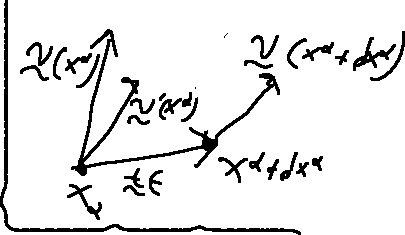
\includegraphics[width=12cm]{2-27-2.png}
	\caption*{Parallel transport}
\end{figure*}
